%% =====================================================================
%% Supplementary Note: stability and support over the operating grid
%%
%% Standalone supplementary section written from module_C2 (branch
%% explore-c2-grid-stability). It does NOT modify the manuscript sources.
%%
%% Compile as-is:   pdflatex supplement_operating_grid.tex
%% To fold into an existing supplement instead, lift the body between
%% \begin{document} and \end{document}; the manuscript already defines \tauc
%% and \lmin, and loads amsmath, graphicx and booktabs.
%% =====================================================================
\documentclass[11pt]{article}
\usepackage[margin=1in]{geometry}
\usepackage{amsmath,amssymb}
\usepackage{graphicx}
\usepackage{booktabs}
\usepackage{microtype}
\usepackage[hidelinks]{hyperref}
\providecommand{\tauc}{\ensuremath{\tau_C}}
\providecommand{\lmin}{\ensuremath{\ell_{\min}}}
\graphicspath{{../figures/}}
\renewcommand{\thesection}{S\arabic{section}}
\renewcommand{\thetable}{S\arabic{table}}
\renewcommand{\thefigure}{S\arabic{figure}}
\title{Supplementary Note: stability and support over the\\ region-calling operating grid}
\date{}
\begin{document}
\maketitle

\section{Motivation and what is being measured}

The region-calling step has two nuisance parameters: the C-score threshold \tauc\ and
the minimum region size \lmin. Reporting a single operating point invites the
objection that the result was chosen; selecting the cell that maximises the number of
significant regions would reintroduce, at the grid level, exactly the multiple-testing
problem the region-level FDR controls within a cell. A natural response is to
\emph{integrate} over a grid $\mathcal{G}$ of operating points and report, for each
locus, the fraction of cells in which it survives.

We evaluated this idea on the stickleback data and on the Nemo simulations. Four
quantities are easily conflated, and we distinguish them throughout:

\begin{enumerate}\itemsep2pt
\item \textbf{Detection stability} --- the fraction of grid cells in which a locus is
      still called as a region.
\item \textbf{Significance stability} --- the fraction of cells in which the called
      region additionally passes the location-matched region-level test ($q_R<0.05$
      against the permutation null, Benjamini--Hochberg-adjusted within that cell).
\item \textbf{Genome-wide count FDR} --- $\mathbb{E}[\#\text{null regions}]/\#\text{observed
      regions}$ at a cell, used to pick an operating point; not per-region.
\item \textbf{The location-matched $p_R$ and $q_R$ at one operating point} --- the test
      that actually carries formal error control.
\end{enumerate}

Quantities 1 and 2 are \emph{robustness rankings}. Neither is a $p$-value, and
neither confers false-discovery control across the grid; error control continues to
come from quantity 4.

\section{The significance layer is redundant with detection}
\label{sec:redundant}

Across the full $25\times7=175$-cell grid ($\tauc=0.02,0.04,\dots,0.50$;
$\lmin\in\{1,2,3,5,10,15,20\}$), the $17$ reported EMMAX regions, and four
region-matching rules, the number of cells in which a region is \emph{detected but not
location-matched significant} is \textbf{zero}. Repeating the analysis on every
null-restricted grid of Section~\ref{sec:admissible} gives the same answer in all
$19$ grid $\times$ matching configurations tested: $0$ discordant cells.

The mechanism is a resolution effect, not a biological one. With $B=200$
permutations the empirical $p$-value floor is $1/(B+1)=0.00498$, and $27.8\%$ of all
region$\times$cell combinations sit exactly at that floor because the
among-population permutation seldom rebuilds an observed locus at its own position.
Benjamini--Hochberg is a step-up procedure, so a set of $k$ regions tied at the floor
$p_0$ is rejected \emph{en bloc} as soon as $p_0\le\alpha k/m$; ties rescue one
another. Where \lmin\ is large the cell tests only one to three regions and BH is
trivially permissive. Either way, among detected cells the raw empirical $p$ is
already below $0.05$ in $100\%$ of cases and BH demotes none.

\textbf{Consequence.} On these data the ``second-tier'' score is numerically identical
to detection stability. It should not be presented as a second inferential tier, nor
described as integrating significance, and the colour scale of any figure built from
it should be labelled as \emph{support}, not significance.

\section{Null behaviour over the operating grid}

We characterised the null directly: for every cell and every one of the $B=200$
among-population permutation surrogates, regions were built with the same LD graph and
the same region rules used for the observed data. Let
$p_{\text{null}}(g)=\Pr_0(N_{\text{regions},g}>0)$.

Three features matter (Fig.~\ref{fig:nulllandscape}; Table~\ref{tab:admissible}).

\paragraph{There is no null-silent corner.} $p_{\text{null}}$ ranges from $0.025$ to
$0.755$ and is \textbf{never zero} on any of the $175$ cells. Some fraction of
surrogates produces at least one LD-supported region everywhere in the parameter
space.

\paragraph{The lenient axis is \lmin, not \tauc.} Spearman correlation of
$p_{\text{null}}$ with \lmin\ is $-0.970$; with \tauc\ it is only $-0.216$. Across the
entire \tauc\ range at $\lmin=1$, $p_{\text{null}}$ falls merely from $0.755$ to
$0.395$ and never approaches any tolerance one might set. The ``lenient corner'' is in
fact a horizontal band: any null-based restriction is close to a minimum-region-size
requirement under another name.

\paragraph{There is no natural break.} Sorted across cells, $p_{\text{null}}$ has a
median gap between adjacent values of $0.0000$ and a largest gap of $0.045$. It is a
smooth continuum, so a cut point is \emph{imposed} rather than discovered.

\begin{figure}[t]\centering
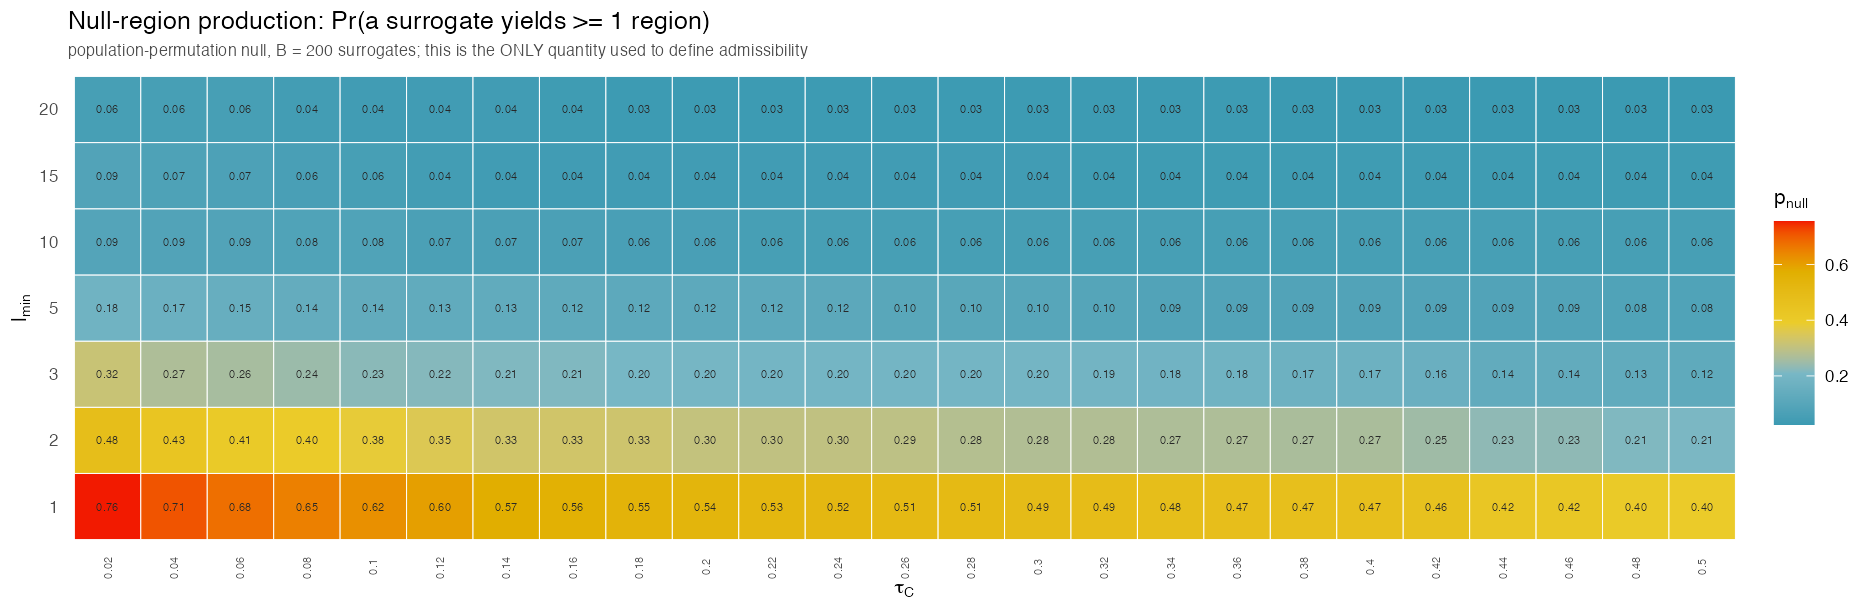
\includegraphics[width=\textwidth]{fig7_null_p_any.png}
\caption{Probability that a permutation surrogate yields at least one region, over the
$\tauc\times\lmin$ grid ($B=200$). The gradient runs almost entirely along \lmin;
no cell reaches zero. Companion panels show the mean null region count
(\texttt{fig8}), null marker coverage (\texttt{fig9}) and, on the identical grid, the
observed region count (\texttt{fig10}).}
\label{fig:nulllandscape}
\end{figure}

\section{Null-informed admissible grids}
\label{sec:admissible}

If no single operating point is to be chosen, one may instead let the null
\emph{exclude} cells that frequently manufacture spurious regions, and assess signals
over what remains:
\[
  \mathcal{G}_{\mathrm{adm}}(\epsilon)=\{g:\ p_{\text{null}}(g)\le\epsilon\}.
\]
Critically, this rule depends on null behaviour only; the empirical region burden was
computed for diagnosis but never consulted in defining admissibility. (The two do
covary strongly --- Spearman $0.925$ between $p_{\text{null}}$ and the observed region
count --- which is precisely why the empirical side must be kept out of the rule.)

\begin{table}[t]\centering
\caption{Candidate null-only admissibility rules on the $175$-cell grid. ``CP'' is the
Clopper--Pearson upper confidence bound for $p_{\text{null}}$ at $B=200$. Every
retained set is a single connected component and a contiguous high-\tauc\ suffix
within each retained \lmin.}
\label{tab:admissible}
\begin{tabular}{lrlr}
\toprule
Rule & Cells retained & \lmin\ retained & Max $p_{\text{null}}$ retained\\
\midrule
$p_{\text{null}}\le0.20$        & 116 & 3, 5, 10, 15, 20 & 0.200\\
$p_{\text{null}}\le0.10$        &  86 & 5, 10, 15, 20    & 0.100\\
$p_{\text{null}}\le0.05$        &  42 & 15, 20           & 0.045\\
CP upper bound $\le0.10$        &  61 & 10, 15, 20       & 0.055\\
CP upper bound $\le0.05$        & \textbf{0} & ---       & ---\\
mean null coverage $\le0.001$   & 107 & all              & 0.470\\
mean null regions $\le0.5$      &  81 & 5, 10, 15, 20    & 0.085\\
\bottomrule
\end{tabular}
\end{table}

\paragraph{Finite $B$ is the binding constraint.} At $\epsilon=0.05$ the point-estimate
rule retains $42$ cells but the confidence-bound rule retains \textbf{none}: not one
cell on the grid can be \emph{shown}, at $B=200$, to have $p_{\text{null}}\le0.05$. At
$\epsilon=0.10$, $25$ of the $86$ retained cells ($29\%$) are statistically
indistinguishable from failing the rule. A cell observed at $20/200$ has a
Clopper--Pearson interval of $[0.062,0.150]$, so $\epsilon=0.05$ and $\epsilon=0.10$
cannot be told apart with this null. Only $\epsilon=0.20$ is reasonably resolved
($13\%$ ambiguous).

\section{Support of the reported regions across admissible grids}

For a prespecified region $r$ we report \emph{detection support}
\[
  D_r=\frac{\#\{g\in\mathcal{G}_{\mathrm{adm}}:\ r\ \text{recovered in}\ g\}}
           {|\mathcal{G}_{\mathrm{adm}}|},
\]
with the denominator running over \emph{all} admissible cells, including those in
which nothing is detected. Regions are fixed \emph{before} the grid search, as the
region set at the reference point $(\tauc,\lmin)=(0.05,3)$, and retained as
member-marker vectors; a region is recovered in a cell when some called region returns
at least half of its markers. Physical-span overlap is not used, because two
physically overlapping components need not be the same LD-defined signal.

\begin{table}[t]\centering
\caption{Detection support of the $17$ reported regions under progressively stricter
null tolerances. The reference point $(0.05,3)$ supplies the displayed boundaries
only; it is not a grid cell and does not define admissibility.}
\label{tab:support}
\begin{tabular}{lrrrr}
\toprule
Region & full grid & $\epsilon=0.20$ & $\epsilon=0.10$ & CP $\le0.10$\\
       & (175 cells) & (116) & (86) & (61)\\
\midrule
Chr5:2.48--2.50\,Mb            & 0.149 & \textbf{0.121} & \textbf{0.116} & \textbf{0.049}\\
Chr1:21.50--21.93\,Mb (inversion) & 0.120 & \textbf{0.103} & \textbf{0.105} & \textbf{0.049}\\
Chr20:0.18--0.26\,Mb           & 0.120 & \textbf{0.103} & \textbf{0.105} & \textbf{0.049}\\
Chr7:11.55--11.66\,Mb          & 0.091 & 0.060 & 0.047 & 0.016\\
Chr4:12.81\,Mb (\emph{Eda})    & 0.069 & 0.034 & 0.035 & 0.016\\
Chr12:16.52--16.55\,Mb         & 0.074 & 0.034 & 0.012 & 0\\
Chr17:9.94\,Mb                 & 0.074 & 0.034 & 0.012 & 0\\
Chr4:27.55\,Mb                 & 0.171 & 0.026 & 0     & 0\\
Chr17:6.55--6.77\,Mb           & 0.069 & 0.026 & 0     & 0\\
Chr20:8.89--8.90\,Mb           & 0.051 & 0.026 & 0.023 & 0\\
Chr18:5.61\,Mb                 & 0.109 & 0.017 & 0     & 0\\
Chr4:22.51\,Mb                 & 0.143 & 0.009 & 0     & 0\\
Chr12:15.55\,Mb                & 0.057 & 0.009 & 0     & 0\\
Chr1:27.28\,Mb                 & 0.063 & 0     & 0     & 0\\
Chr20:3.67\,Mb                 & 0.051 & 0     & 0     & 0\\
Chr3:13.03\,Mb                 & 0.034 & 0     & 0     & 0\\
Chr4:25.67--25.99\,Mb          & 0.034 & 0     & 0     & 0\\
\midrule
Regions with zero support      & 0/17 & 4/17 & 9/17 & 12/17\\
Spearman vs.\ full grid        & 1.000 & 0.654 & 0.404 & 0.477\\
\bottomrule
\end{tabular}
\end{table}

Table~\ref{tab:support} shows that tightening the tolerance does not merely re-rank
the regions. At $\epsilon=0.05$ (and under the null-coverage rule) \emph{all $17$}
reported regions lose their support entirely. The reason is mechanical rather than
evidential: nine of the seventeen regions contain four SNPs or fewer, so once
admissibility requires $\lmin\ge10$ they can be recovered only by merging into a
larger component. A filter that deletes the entire reported region set is not
sharpening the inference.

\paragraph{Corroboration of the null rule.} The regions that drop out are the ones the
rule is meant to remove. Computed \emph{after} the rule was fixed, and never used to
construct it: the four regions losing all support at $\epsilon=0.20$ are detected only
in cells of mean $p_{\text{null}}=0.488$, with $0\%$ of their detecting cells
admissible; the thirteen regions retaining support are detected in cells of mean
$p_{\text{null}}=0.361$, with $5$--$57\%$ of their detecting cells admissible.

\paragraph{Tolerance-robust signals.} Only three regions retain support under every
tolerance examined: \textbf{Chr5:2.48--2.50\,Mb}, the \textbf{Chr1 inversion}, and
\textbf{Chr20:0.18--0.26\,Mb}. \emph{Eda} survives $\epsilon=0.20$ but not the
confidence-bound rule. All remaining regions are tolerance-dependent.

\section{Robustness of the summary itself}

\paragraph{Matching rule.} Requiring $25\%$, $50\%$ or $75\%$ of a region's markers to
be returned gives closely agreeing rankings (Spearman $0.776$, $1.000$, $0.972$
against the $50\%$ rule); a reciprocal variant that also caps how much larger the
matched region may be gives $0.880$. The retention threshold is not a sensitive
choice. Permissive ``any shared marker'' or physical-overlap matching \emph{is}
different, because it lets a region be credited when it has been swallowed into a
chromosome-scale component at low \tauc.

\paragraph{Reference point.} Redefining the displayed regions at neighbouring points
--- $(0.04,3)$, $(0.06,3)$, $(0.05,2)$, $(0.05,5)$ --- changes the inventory
substantially ($8$ to $23$ regions; $0$ to $9$ of them with zero support) but not the
conclusion: Chr5:2.48--2.50\,Mb is the best-supported region at four of the five
reference points, with an identical maximum support of $0.121$.

\paragraph{Grid range and density.} Support is not invariant to grid design.
Restricting to $\tauc>0.26$ sends every region to zero, whereas restricting to
$\tauc\le0.26$ reproduces the full-grid ranking exactly (Spearman $1.000$): all of the
information lives in the permissive half, and lengthening the \tauc\ range dilutes
every score by inflating the denominator alone. A coarser but defensible grid
($5\times5$) drives $13$ of $17$ regions to exactly zero.

\paragraph{Anchor-free check.} Defining marker-level support $S_m$ --- the fraction of
admissible cells in which marker $m$ lies in any region --- and grouping supported
markers into families by the same $r^2$ linkage and $500$\,kb gap rule used for region
calling, we find no signal that the reference point misses: on every admissible grid
each family overlaps a reported region, region- and marker-level support agree at
Spearman $0.992$, and the largest $S_m$ outside the reported set is $0.069$. On the
unrestricted grid $41$ additional families appear, but with a median size of one
marker. We stress that $S_m$ correlates with the marker C-score at Spearman
$0.69$--$0.85$ and is therefore largely a re-expression of it; it is reported as
support, never as independent evidence.

\begin{figure}[t]\centering
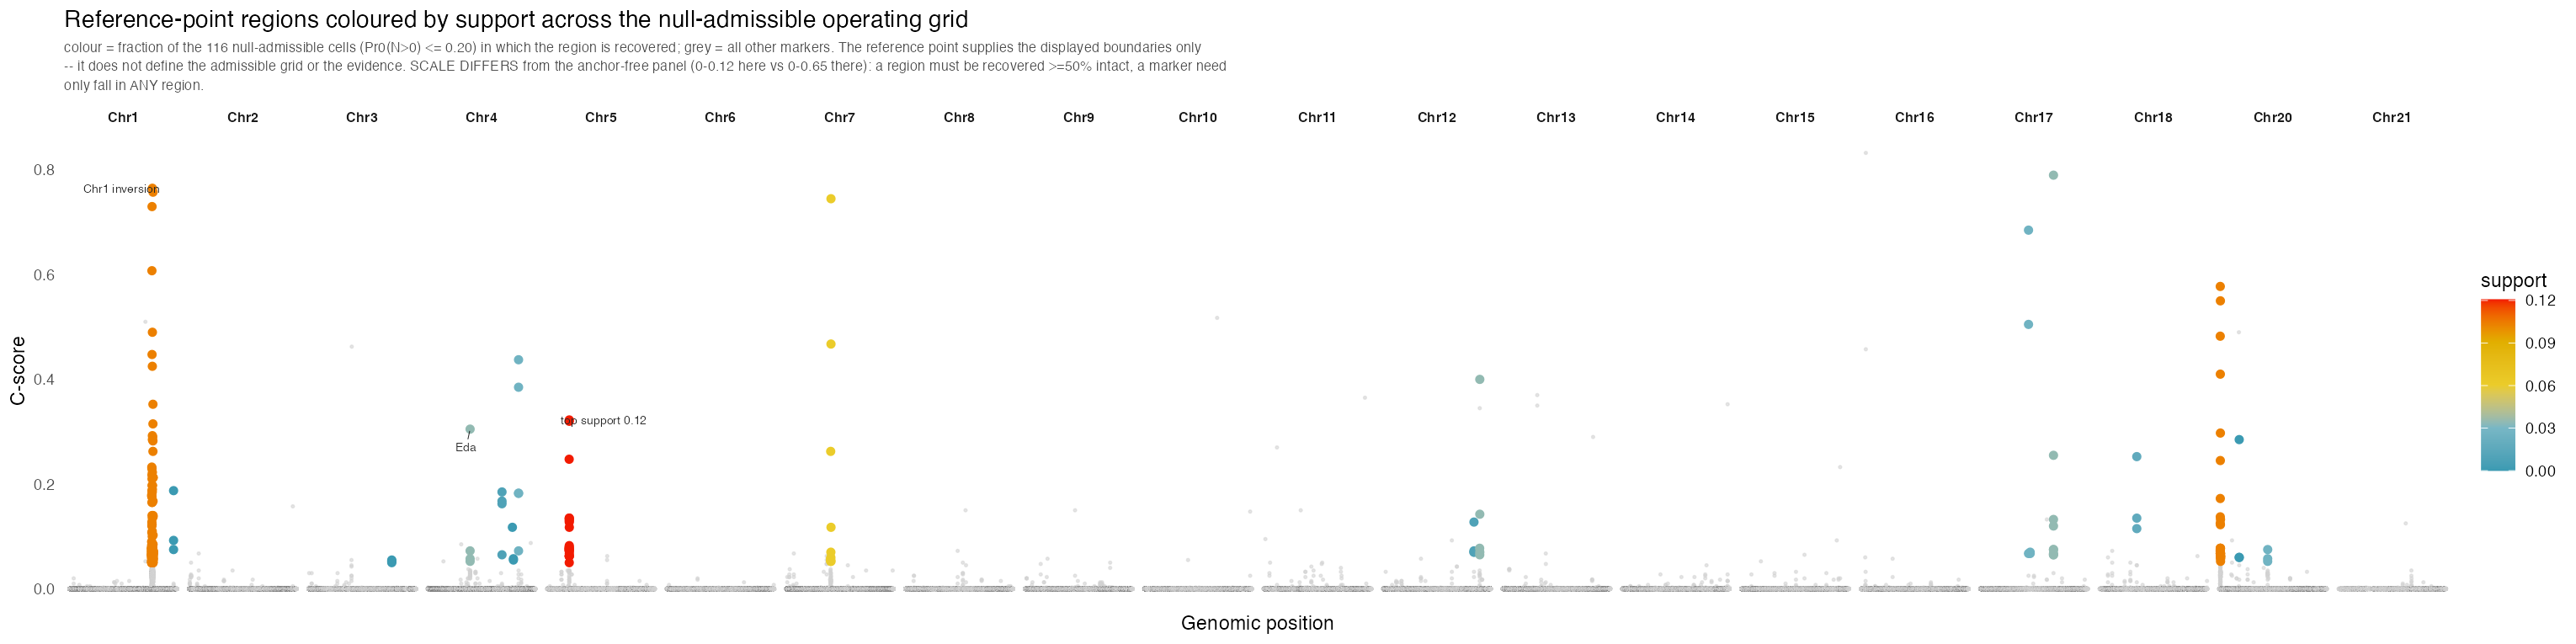
\includegraphics[width=\textwidth]{fig13_manhattan_reference_support_P20_ownscale.png}\\[4pt]
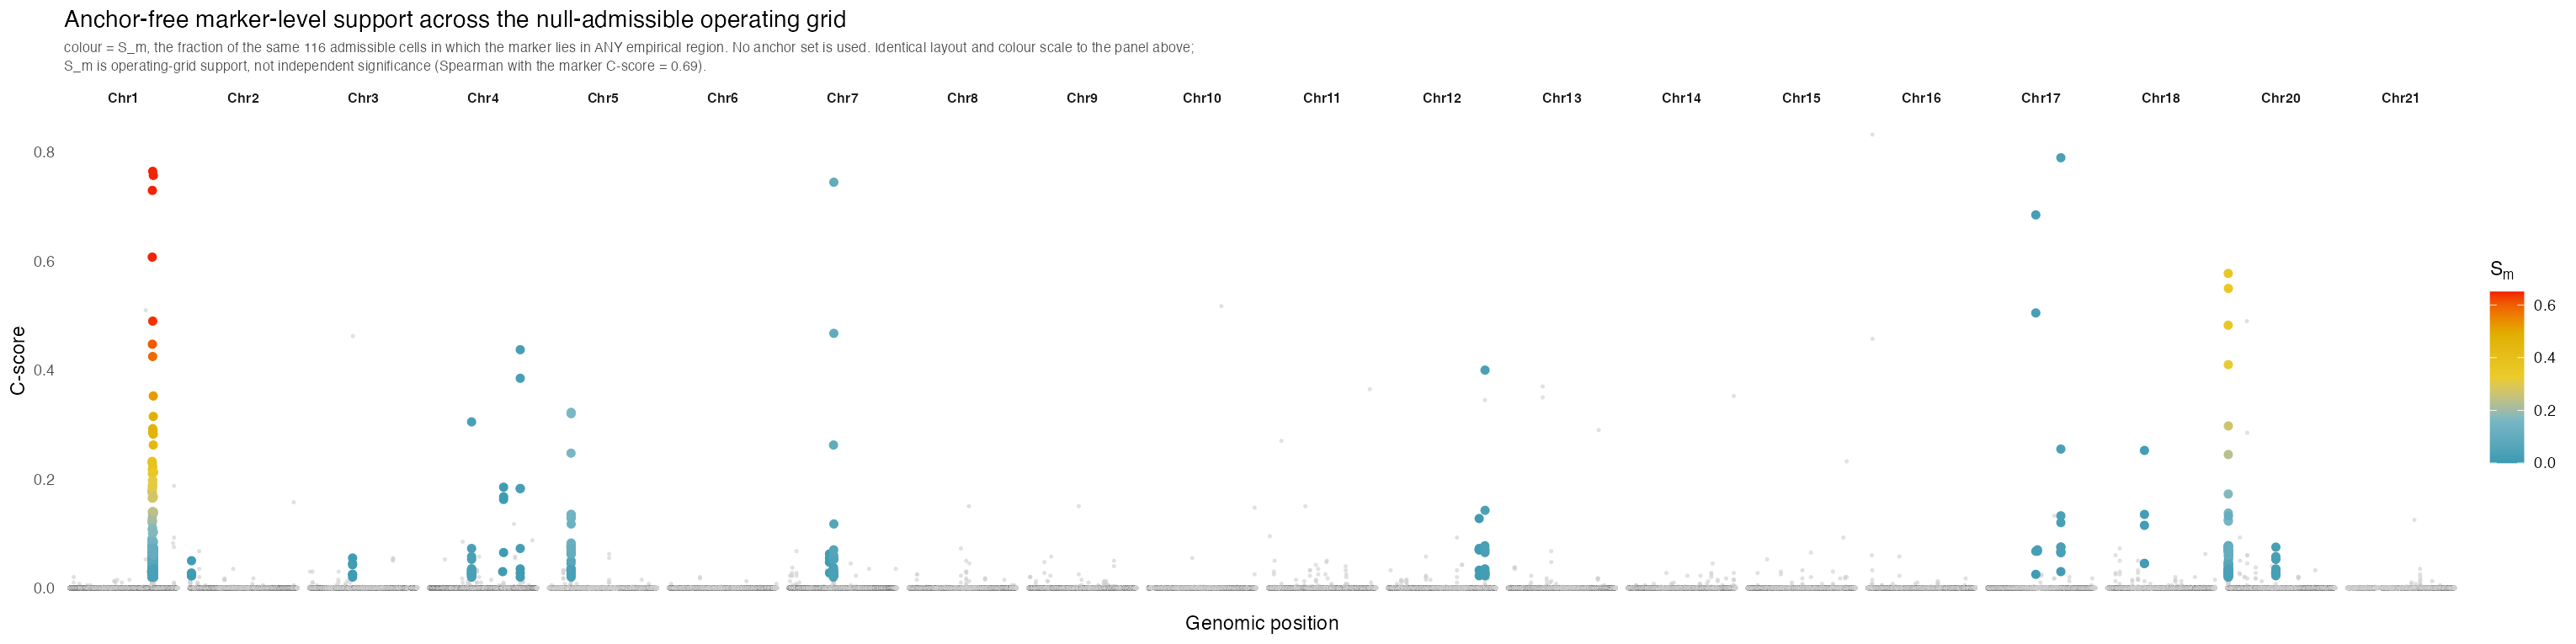
\includegraphics[width=\textwidth]{fig14_manhattan_marker_support_P20.png}
\caption{\textbf{Top:} the reported regions coloured by their support across the
null-admissible grid ($\epsilon=0.20$, $116$ cells); grey, all other markers.
\textbf{Bottom:} the anchor-free companion, every marker coloured by its own $S_m$ on
the same chromosome layout. The colour ranges differ ($0$--$0.12$ against $0$--$0.65$)
because a region must be returned at least half intact whereas a marker need only fall
inside some region; a shared-scale version of the upper panel is provided for direct
side-by-side reading. The colour is detection support, not significance
(Section~\ref{sec:redundant}).}
\label{fig:manhattan}
\end{figure}

\section{Simulation check}

On the Nemo simulations, where region truth is known, grid support does separate true
from false regions: replicate-averaged over five environments, true regions score
$0.437$ against $0.094$ for false ones (Wilcoxon $p\le7\times10^{-4}$ in every
informative replicate). Ranking by support gives a precision--recall AUC of
$0.901\pm0.052$. However, ranking the same regions by a single number requiring no
grid at all --- the maximum marker C-score within the region --- does better,
$0.943\pm0.025$. Detection and significance support are again identical to three
decimal places. The simulations therefore validate the idea but do not motivate it
over a far simpler statistic.

\section{What we claim, and what we do not}

\paragraph{Safe.} High support means a region is insensitive to the stated \tauc\ and
\lmin\ ranges. Low support means it lies near a calling boundary. The summary exposes
parameter sensitivity and reduces reliance on any one cell. Reported support is
meaningless without its grid, null basis, $B$, and matching rule, all of which we
give.

\paragraph{Not claimed.} That grid cells are independent, or that the fraction is a
probability: they are strongly dependent, and $\tauc\le0.26$ alone reproduces the full
ranking. That integrating over the grid controls the false-discovery rate: it does
not, and on these data it does not even add a second criterion beyond detection. That
support is invariant to grid design, or that a null-derived admissibility boundary is
a property of the data rather than of a chosen tolerance. That low support means a
region is false.

\paragraph{Recommended reading of these results.} Because $p_{\text{null}}$ is a smooth
continuum with no break, because the tolerance most would reach for
($\epsilon=0.05$) is unresolvable at $B=200$ and removes every reported region, and
because the axis actually being filtered is \lmin\ --- already an explicit, reported
parameter --- we do not adopt a hard admissibility rule. We retain the single
prespecified operating point with its location-matched $q_R$ as the reported
inference, and present the null landscape together with support at
$\epsilon\in\{0.20,0.10\}$ as a sensitivity analysis, noting that three regions
(Chr5:2.48--2.50\,Mb, the Chr1 inversion, Chr20:0.18--0.26\,Mb) are robust across all
tolerances examined.

\end{document}
